\documentclass[letterpaper,10pt]{report}
\usepackage{textcomp}
\usepackage[utf8]{inputenc}
\usepackage[T1]{fontenc}
\usepackage{fullpage}
\usepackage[spanish, activeacute]{babel}
\usepackage{csquotes}
\usepackage{url}
\usepackage{newcent}
\usepackage{textcomp}
\usepackage{graphicx}
\usepackage{caption}
\usepackage{makeidx}
\usepackage{vmargin}
\usepackage{multirow}

\usepackage{pdfpages}
\usepackage{tabularx}
\usepackage{rotating}
\usepackage{float}
\usepackage{caption}
\usepackage{ragged2e}
\usepackage{listings}
\usepackage{color}
\usepackage[hidelinks]{hyperref}
\usepackage{natbib} %bibliografia
\usepackage[spanish]{babel}
\usepackage{longtable}
\graphicspath{imagenes/}
\makeindex

\begin{document}
	\begin{titlepage}
	\begin{center}
		\sc \LARGE Universidad Polit'ecnica de Pachuca\\
		\bigskip
		
\includegraphics[scale=0.2]{img/logo.png}
	\end{center}
	\bigskip
	\begin{center}
		\huge{Codeland-oop\\}
		\vspace*{1cm}
		\sc \LARGE M. en C. Alicia Oriz Montes\\
		\vspace*{0.5cm}
		\sc \LARGE Proyecto de Investigación\\
		\vspace*{0.5cm}
		\sc \LARGE Integrantes: \\
	    \sc \Large Juan Antonio Ayola Cortes \\
	    \sc \Large Juan Daniel Soto Dimas \\
		\sc \Large Miguel 'Angel Vite Hern'andez \\
		\vfill
		\sc Ingenier'ia en Software
	\end{center}
\end{titlepage}
	\tableofcontents
	\listoffigures
	\listoftables
	\pagenumbering{arabic}
	\chapter{Introducci'on}
La programación orientada a objetos es uno paradigma de suma importancia dentro de la programación por lo que es basico conocerlo, y resulta muy útil que los estudiantes que cursan carreras técnicas o universitarias enfocadas al ámbito de la programación tengan un alto conocimiento de esto, sin embargo a pesar de llevarla como materia, les es difícil aprenderla por los amplios conceptos que maneja. Esto tambien conlleva a otro problema, que es la deserción de los alumnos de la carrera. La reprobación estudiantil es un problema añejo y complejo en las instituciones de educación superior. El propósito de este proyecto es aumentar el egreso de estudiantes.

\section{Problematica}
\subsection{Ingeniería es el área con mayor tasa de abandono escolar universitario, particularmente aquellas vinculadas con la informática}
El mercado laboral sufre el dilema vocacional porque las carreras más demandadas son las menos elegidas por los estudiantes después del primero año, ya que el abandono es mayor en el área de ingeniería y especialmente en informática. El foro profesional de los ingenieros técnicos en España advierte que el déficit de profesionales en el área de software y telecomunicaciones derivará en la importancia masiva de ingenieros dentro de una década.

\subsection{Problemas del aprendizaje de la programación orientada a objetos}
El problema del aprendizaje de la programación orientada a objetos se manifiesta toda vez que es una materia compleja que implica la integración de muchos elementos como son el paradigma orientado a objetos, el lenguaje de programación, el entorno de desarrollo, la metodología de desarrollo, el lenguaje de modelado, los patrones de desarrollo y la lógica de programación. Por lo tanto los alumnos se encuentran ante una cantidad abrumadora de conceptos en un periodo corto de tiempo, lo que dificulta su asimilaci'on y el desarrollo de las habilidades para generar l'ineas de c'odigo como lo explica \cite{spigariol2013ensenando}:

\begin{minipage}{0.9\linewidth}
	 \vspace{5pt}
	 \begin{small}
	 	``Los docentes ve'ian en los estudiantes que el uso del lenguaje representaba una curva de aprendizaje abrupta en los primeros momentos de la materia ya que requieren el manejo de una cantidad 'amplia de conceptos antes de poder realizar algo relativamente sencillo (...). La disociaci'on entre teor'ia y pr'actica que se generaba era ciertamente contraproducente y dificultaba el proceso de aprendizaje."
	 \end{small}
\end{minipage}

Debido a que los conceptos que se tratan en la asignatura de programación orientada a objetos son muchos y en algunos casos difíciles de comprender por el alto nivel de abstracción, esto se configura como un factor que dificulta el aprendizaje, esto se ha visto reflejado por ejemplo cuando los estudiantes generalmente no distinguen entre lo que es una clase y un objeto.

Además la forma de enseñar la asignatura de programación orientada a objetos es muy similar a la de la programación estructurada, primero se tratan temas básicos del lenguaje de programación, como son la declaraciones de los tipos de datos, las estructuras de control y las sentencias de condición, para posteriormente enseñar lo que son las clases, objetos y los principales temas propios del paradigma orientada a objetos, esto contribuye a que los estudiantes sientan que continúan con el mismo paradigma de programación estructurada.

En virtud de que los estudiantes no logran asimilar este cambio de paradigmas, usan el lenguaje de programación orientada a objetos como un lenguaje de programación estructurada, por consiguiente no resuelven problemas diseñando clases.

Así pues los estudiantes al llegar a la asignatura de programación orientada a objetos se enfrentan de entrada a dos problemas, la percepción que tienen de dificultad y por otro lado el proceso de transición del paradigma estructurado hacia el paradigma orientado a objetos.

\section{Objetivo general}
Desarrollar una aplicación móvil con la herramienta de Android Studio, para que las personas interesadas en la programación puedan aprender de una mejor manera el paradigma de programación orientada a objetos, y así puedan adquirir y/o reforzar su conocimiento de este paradigma. 

\section{Objetivos espec'ificos} 
\begin{itemize}
\item Proporcionar a los estudiantes y personas interesadas en la programación, información acerca del paradigma de programación orientada a objetos.
\item Evaluar el conocimiento de los usuarios de la aplicación con exámenes al finalizar un tema.
\item Diseñar una interfaz de tal forma que el usuario pueda aprender a utilizar la aplicación en el menor tiempo posible.
\item Programar la aplicación de tal forma de que no consuma muchos recursos al usarla en un celular.
\end{itemize}

\section{Justificación}
\subsection{Las TIC en la educaci'on}
De acuerdo con \cite{palaciostics} en la educaci'on el uso de las nuevas tecnolog'ias de la informaci'on ha pasado por las siguientes etapas:

\begin{figure}
	\begin{center}
		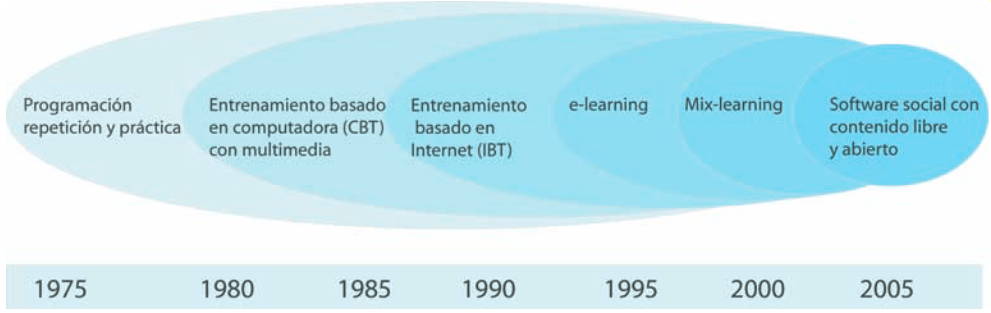
\includegraphics[scale=0.5]{img/img1.png} 
		\caption{Evoluci'on de las TIC en la educaci'on. (Basado en \cite{palaciostics})}
		\label{tic}
	\end{center}
\end{figure}

Esta evoluci'on muestra como cada vez el aprendizaje va utilizando m'as tecnolog'ia; pasando de ser 'esta simplemente una herramienta de apoyo, hasta ser la plataforma a trav'es de la cual se presentan los contenidos y eval'uan los conocimientos. 

Mix-Learning. La etapa posterior al e-learning es la aplicaci'on de una mezcla de sus herramientas con sistemas educativos tradicionales. La finalidad es dirigir m'as espec'ificamente los contenidos a los estudiantes. Es as'i que el Blend Learning, Mix Learning o Hybrid Learning se presenta como ``la combinaci'on efectiva de los diferentes modelos de reparto, modelos de ense'nanza y modelos de aprendizaje" \citep{olivares2016tic}.

\subsection{M-Learning en la educaci'on}
Seg'un la Organizaci'on de las Naciones Unidas para la Educaci'on la Ciencia y la Cultura \citep{dykes2012mobile} existen 5.9 billones de suscripciones de tel'efonos m'oviles en el mundo, contra los 7.04 billones de habitantes. Adem'as, en el a'no 2020 los dispositivos m'oviles ser'an la principal herramienta de conexi'on a internet para la mayor'ia de la poblaci'on; en Jap'on, actualmente el 75\% de su poblaci'on tiene un dispositivo m'ovil como primer medio de acceso a internet \citep{camacho2011m}. 

Asimismo, en a'nos recientes el uso de la tecnolog'ia m'ovil para fines educativos, conocido como m-learning, ha tenido un gr'an desarrollo en la educaci'on superior, ya que existen universidades de Europa y Am'erica que cuentan con sistemas de educaci'on m'ovil \citep{traxler2007defining}.

\subsection{La importancia de la programaci'on orientada a objetos}
La programaci'on Orientada a Objetos surge como el paradigma que permite manejar ampliamente las nuevas plataformas que garanticen desarrollar aplicaciones robustas, portables y reutilizables que puedan ofrecer una soluci'on a largo plazo en un mundo donde los cambios se dan a cada momento.

El desarrollo de programas orientados a objetos es un enfoque diferente del mundo inform'atico. Implica la creaci'on de modelos del mundo real y la construcci'on de programas inform'aticos basados en esos modelos.

La importancia de esta programaci'on radica en que, favorece la creaci'on de programas de calidad, fuerza en mantenimiento, en extensi'on y reutilizaci'on de programas. Est'a basada en el modo de pensar del hombre y en el modo de trabajar de la m'aquina.

Es muy importante que los estudiantes sean capaces, no s'olo de manejar los conceptos de orientaci'on a objetos, sino tambi'en de aplicarlos de manera efectiva en el desarrollo de programas.
	\chapter{Estado del arte}
Aplicaciones existentes para aprender programación orientada a objetos:
\begin{longtable}[c]{|l|l|l|l|l|l|}
\hline
\rowcolor[HTML]{34CDF9} 
{\color[HTML]{FFFFFF} Nombre}                                              & {\color[HTML]{FFFFFF} Temas}                                                                                                                                                                                                                                                                                                                                                                                                 & {\color[HTML]{FFFFFF} Juegos} & {\color[HTML]{FFFFFF} Tamaño} & {\color[HTML]{FFFFFF} Idioma} & {\color[HTML]{FFFFFF} Test} \\ \hline
\endfirsthead
%
\endhead
%
\begin{tabular}[c]{@{}l@{}}Programación\\ Orientada a Objetos\end{tabular} & \begin{tabular}[c]{@{}l@{}}-Tipo de dato anónimo\\   -Tipo abstracto\\   -SOLID\\   -RAII\\   -Proxy\\   -Programación basada en prototipos\\   -Problema del diamante\\   -Principio de sustitución de Liskov\\   -Principio de segregación de la inerfaz\\   -Principio de responsabilidad única-Objeto\\   -Método\\   -Metaclase\\   -Encapsulamiento\\   -Destructor\\   -Delegación\\   -Clase\\   -Campo\end{tabular} & No                            & 3.87M                         & Español                       & No                          \\ \hline
\begin{tabular}[c]{@{}l@{}}Object\\ Oriented Programming\end{tabular}      & \begin{tabular}[c]{@{}l@{}}-Object\\   -Class\\   -Constructor\\   -Destructor\\   -Get\\   -Set\\   -toString\\   -Private Method\\   -Protected Method\\   -Public Method\\   -Inheritance\\   -Interfaces\\   -Adbstrct\\   -Plymorphism\\   -Encapsulation\end{tabular}                                                                                                                                                  & No                            & 9.64M                         & Ingles                        & No                          \\ \hline
\begin{tabular}[c]{@{}l@{}}Object\\ Oriented Programming\end{tabular}      & \begin{tabular}[c]{@{}l@{}}-OOP in PHP - What is Object\\   -OOP in PHP - Intro to Class\\   -OOP in PHP - Inheritance\\   -OOP in PHP - Interfaces\\   -OOP in PHP - Abstract\\   -OOP in PHP - Constructor\\   -OOP in PHP - Polymorphism\\   -OOP in PHP - Encapsulation\\   -OOP in PHP - Destructor\\   -OOP in PHP - Private Method\\   -OOP in PHP - Protected Method\\   -OOP in PHP - Public Method\end{tabular}    & No                            & 9.71M                         & Ingles                        & No                          \\ \hline
\begin{tabular}[c]{@{}l@{}}Object\\ Oriented Programming\end{tabular}      & \begin{tabular}[c]{@{}l@{}}-Introduction to Object.\\   -Class in OOP and its detail with syntax code.\\   -Abstraction concepts in OOP\\   -What is Polymorphism in OOP\\   -Inheritance concepts with syntax code.\\   -Method overloading vs. overriding\\   -Encapsulation concept\\   -Keywords in java\\   -Constructor in Java etc…\\   -Java Programming Statements with code syntax.\end{tabular}                   & No                            & 2.8M                          & Ingles                        & No                          \\ \hline
OPP for Beginners                                                          & \begin{tabular}[c]{@{}l@{}}-Naming convention\\   -Object and class\\   -Method overloading\\   -Constructor\\   -Static keyword\\   -Inheritance\\   -Aggregation\\   -Method overrridong\\   -covariant return type\\   -Abstract class\\   -Package \\ -object class\end{tabular}                                                                                                                                         & No                            & 8.1M                          & Ingles                        & Si                          \\ \hline
\caption{Tabla comparativa de las distintas aplicaciones para aprender programación orientada a objetos.}
\label{aplicaciones}\\
\end{longtable}
	\chapter{Marco teórico}

\section{Programación Orientada a Objetos}
La programación orientada a objetos, ha tomado las mejores ideas de la programación estructurada y los ha combinado con varios conceptos nuevos y potentes que incitan a contemplar las tareas de programación desde un nuevo punto de vista. La programación orientada a objetos, permite descomponer más fácilmente un problema en subgrupos de partes relacionadas del problema. Entonces, utilizando el lenguaje se pueden traducir estos subgrupos a unidades auto contenidas llamadas objetos.. \citep{izquierdo2007introduccion}.

\subsection{Objeto}
Una estructura de datos y conjunto de procedimientos que operan sobre dicha estructura. Una definición más completa de objeto es: una entidad de programa que consiste en datos y todos aquellos procedimientos que pueden manipular aquellos datos; el acceso a los datos de un objeto es solamente a través de estos procedimientos, únicamente estos procedimientos pueden manipular, referenciar y/o modificar estos datos.

Para poder describir todos los objetos de un programa, conviene agrupar éstos en clases \citep{izquierdo2007introduccion}.

\subsection{Clase}
Podemos considerar una clase como una colección de objetos que poseen características y operaciones comunes. Una clase contiene toda la información necesaria para crear nuevos objetos \citep{izquierdo2007introduccion}.

\subsection{Encapsulación}
Es una técnica que permite localizar y ocultar los detalles de un objeto. La encapsulación previene que un objeto sea manipulado por operaciones distintas de las definidas. La encapsulación es como una caja negra que esconde los datos y solamente permite acceder a ellos de forma controlada \citep{izquierdo2007introduccion}.

\subsection{Abstracción}
En el sentido más general, una abstracción es una representación concisa de una idea o de un objeto complicado. En un sentido más específico, la abstracción localiza y oculta los detalles de un modelo o dise'no para generar y manipular objetos \citep{izquierdo2007introduccion}. 

\subsection{Objetos}
Un objeto es una entidad lógica que contiene datos y un código que manipula estos datos; el enlazado de código y de datos, de esta manera suele denominarse encapsulación. Cuando se define un objeto, se está creando implícitamente un nuevo tipo de datos \citep{izquierdo2007introduccion}.

\subsection{Polimorfismo}
Esta característica es la capacidad que objetos similares tienen para responder de
diferentes formas al mismo mensaje, y permite al programador implementar
múltiples formas de un mismo método, dependiendo cada una de ellas de la clase
sobre la que se realice la implementación. Esto permite acceder a varios métodos
distintos utilizando el mismo medio de acceso (el mismo nombre). El polimorfismo
está muy relacionado con la herencia \citep{velarde2006introduccion}.

\subsection{Herencia}
Según \cite{joyanes1996programacion}, la herencia “Es la capacidad para crear nuevas
clases de objetos que se construyen basados en clases existentes”. La herencia
es una propiedad que permite a un objeto poseer propiedades de otras clases.
Además, a estos nuevos objetos creados es posible asignarles nuevos atributos
y métodos.

La clase que puede ser heredada se denomina clase base (superclase) y la clase
que hereda se denomina clase derivada (subclase) \citep{velarde2006introduccion}.

\subsection{Atributos}
Describen las características de los objetos: tipo de acceso (privado, protegido, publico) y tipo de dato (entero, real, booleano, etcétera) \citep{izquierdo2007introduccion}. 

\subsection{Métodos}
Describen lo que puede hacer la clase; es decir, el método define las instrucciones necesarias para realizar un proceso o tarea específicos. La definición del método se compone de tipo de acceso, tipo de retorno, nombre del método, parámetros, si los requiere, y el cuerpo del método \citep{izquierdo2007introduccion}.

\section{Programación}

\subsection{Programa}
Un programa es una secuencia lógica de instrucciones escritas en un determinado lenguaje de programación que dicta a la computadora las acciones que debe llevar a cabo.

\subsection{Tipo de dato}
Es la representación simbólica de un atributo de una entidad; en programación, los datos expresan características de las entidades sobre las que opera un algoritmo. Los datos representan hechos, observaciones, cantidades o sucesos y pueden tomar la forma de números, letras o caracteres especiales \citep{izquierdo2007introduccion}.

\subsection{Algoritmo}
Se define como una técnica de solución de problemas que consiste en una serie de instrucciones paso por paso y que produce resultados específicos para un problema determinado \citep{izquierdo2007introduccion}. 

\subsection{Variable}
Es un área de almacenamiento temporal a la que se ha asignado un nombre simbólico y cuyo valor puede ser modificado a lo largo de la ejecución de un programa \citep{izquierdo2007introduccion}. 

\subsection{Constante}
Es un valor definido que no cambia durante la ejecución de un programa \citep{izquierdo2007introduccion}. 

\subsection{Parámetros formales}
Son variables que reciben valores desde el punto de llamada que activa al método \citep{izquierdo2007introduccion}.


\section{Herramientas de Desarrollo}
\subsection{Java}
Java es uno de los lenguajes de programación más populares del mundo. Es un lenguaje orientado a objetos, potente, versátil y mutiplataforma (corre en cualquier sistema operativo moderno). Java fue elegido como el lenguaje para el entorno de desarrollo de Android, el sistema operativo móvil líder en smartphones y tablets \citep{izquierdo2007introduccion}.

\subsection{Android}
Android es un sistema operativo inicialmente pensado para teléfonos móviles, al igual que iOS, Symbian y Blackberry OS. Lo que lo hace diferente es que está basado en Linux, un núcleo de sistema operativo libre, gratuito y multiplataforma \citep{studio2016conoce}.

\subsection{SQLite}
SQLite es un sistema de gestión de bases de datos relacional compatible con ACID, contenida en una relativamente pequeña (~275 kiB) biblioteca escrita en C \citep{owens2010sqlite}.


\subsection{Git}
Git es un sistema de control de versiones distribuido cuyo objetivo es el de permitir mantener una gran cantidad de código a una gran cantidad de programadores eficientemente \citep{alvarez2014introduccion}.

\subsection{Android Studio}
Es el entorno de desarrollo integrado (IDE) oficial para el desarrollo de aplicaciones para Android y se basa en IntelliJIDEA \citep{studio2016conoce}.
\subsection{Metodologia}
Conjunto de métodos que se siguen en una investigación científica, un estudio o una exposición doctrinal
\subsection{Metodologia SCRUM}
SCRUM es un marco de trabajo iterativo, incremental para el desarrollo de proyectos, productos y aplicaciones.Estructura el desarrollo en ciclos de trabajo llamados sprints.
\section{Herramientas de Diseño}

\subsection{UML}
UML son las siglas de “Unified Modeling Language” o “Lenguaje Unificado de Modelado”. Se trata de un estándar que se ha adoptado a nivel internacional por numerosos organismos y empresas para crear esquemas, diagramas y documentación relativa a los desarrollos de software.

\subsection{Material Design}
Material Design es un concepto, una filosofía, unas pautas enfocadas al diseño utilizado en Android.

	\chapter{Desarrollo}
Este proyecto se desarrollará con la metodología SCRUM con 8 sprints de una revision por semana, haciendo uso de historias de usuario y de la grafica del quemado para llevar un control de que historias de usuario se quemaron.

\section{Recursos}
\subsection{Recursos humanos}
\begin{table}[H]
\centering
\begin{tabular}{|l|l|l|}
\hline
Rol               & Personas requeridas & Salario  \\ \hline
Programador       & 1                   & \$15,000 \\ \hline
Diseñador         & 1                   & \$10,000 \\ \hline
Tester            & 1                   & \$10,000 \\ \hline
Lider de proyecto & 1                   & \$15,000 \\ \hline
\end{tabular}
\caption{Tabla del pesonal requerido.}
\label{personal}
\end{table}

\subsection{Recursos materiales}
\begin{table}[H]
\centering
\begin{tabular}{|l|l|l|}
\hline
Equipo          & Precio  & Unidades necesarias \\ \hline
Computadoras    & \$8,000 & 2                   \\ \hline
Celular Android & \$5,000 & 1                   \\ \hline
\end{tabular}
\caption{Tabla de recursos materiales.}
\label{materiales}
\end{table}

\subsection{Recursos tecnológicos}
\begin{table}[H]
\centering
\begin{tabular}{|l|l|}
\hline
Concepto       & Precio  \\ \hline
GanttProject   & \$0 \\ \hline
Pencil         & \$0 \\ \hline
Android Studio & \$0 \\ \hline
\end{tabular}
\caption{Tabla de recursos tecnológicos}
\label{tecnologicos}
\end{table}

\subsection{Recursos administrativos}
\begin{table}[H]
\centering
\begin{tabular}{|l|l|}
\hline
Concepto     & Precio       \\ \hline
Agua         & \$100 al mes \\ \hline
Electricidad & \$300 al mes \\ \hline
Internet     & \$500 al mes \\ \hline
\end{tabular}
\caption{Tabla de recursos administrativos}
\label{administrativos}
\end{table}

\section{Diagrama de Gantt}
\begin{figure}[H]
	\begin{center}
		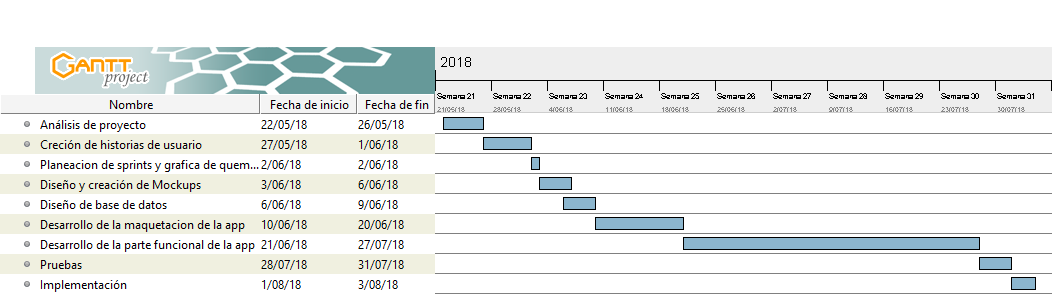
\includegraphics[scale=0.6]{img/cronograma.png} 
		\caption{Cronograma de actividades a seguir.}
		\label{gantt}
	\end{center}
\end{figure}

\section{Historias de usuario}

\begin{table}[H]\small
\begin{tabular}{@{\extracolsep{\fill}} | p{5cm} | p{5cm} | p{5cm} | }
\multicolumn{3}{|c|}{1. Aplicación didactica} \\ \hline
  \hline
\multicolumn{3}{|p{15cm}|}{Como usuario quisiera que la aplicación fuera de un modo didáctica y de aprendizaje mediante ejercicios.} \\ \hline
\hline
Estimaci'on: 7 &semanas	Valor: 50	& Dependencias: \\
\hline
\multicolumn{3}{|p{15cm}|}{Condiciones de satisfacci'on:
\begin{itemize}
	\item La aplicación contendrá información selecta y bien explicada.
	\item Se incluirán algunos ejercicios los cuales deberán resolverse en la computadora.
\end{itemize}
}\\ \hline
\hline
\end{tabular}
\caption{Historia de usuario 1}
\label{hu1}
\end{table}
%%%%%%%%%%%%%%%%%%%%%%%%%%%%%%%%%%%%%%%%%%%%%%%%%%%%%%%%%%%%%%%%%%%%%%%%%%%%%%%%%%%%%%
\begin{table}[H]\small
\begin{tabular}{@{\extracolsep{\fill}} | p{5cm} | p{5cm} | p{5cm} | }
\multicolumn{3}{|c|}{2. Explicaciónes detalladas} \\ \hline
  \hline
\multicolumn{3}{|p{15cm}|}{Como usuario quisiera que explicara a detalle cómo hacer las cosas y para que podrían servir.} \\ \hline
\hline
Estimaci'on: 7 &semanas	Valor: 60	& Dependencias: \\
\hline
\multicolumn{3}{|p{15cm}|}{Condiciones de satisfacci'on:
\begin{itemize}
	\item Se dará una aplicación detallada de cada tema así como ejemplos de uso.
\end{itemize}
}\\ \hline
\hline
\end{tabular}
\caption{Historia de usuario 2}
\label{hu2}
\end{table}
%%%%%%%%%%%%%%%%%%%%%%%%%%%%%%%%%%%%%%%%%%%%%%%%%%%%%%%%%%%%%%%%%%%%%%%%%%%%%%%%%%%%%%
\begin{table}[H]\small
\begin{tabular}{@{\extracolsep{\fill}} | p{5cm} | p{5cm} | p{5cm} | }
\multicolumn{3}{|c|}{3. Modalidad de juegos} \\ \hline
  \hline
\multicolumn{3}{|p{15cm}|}{Como usuario quisiera que la aplicación tuviera la modalidad de juegos, con breves capsulas que expliquen la teoría.} \\ \hline
\hline
Estimaci'on: 6 &semanas	Valor: 60	& Dependencias: \\
\hline
\multicolumn{3}{|p{15cm}|}{Condiciones de satisfacci'on:
\begin{itemize}
	\item Se pondrá información sobre algunos conceptos y se hará un pequeño test de manera que ayude a recordar.
\end{itemize}
}\\ \hline
\hline
\end{tabular}
\caption{Historia de usuario 3}
\label{hu3}
\end{table}
%%%%%%%%%%%%%%%%%%%%%%%%%%%%%%%%%%%%%%%%%%%%%%%%%%%%%%%%%%%%%%%%%%%%%%%%%%%%%%%%%%%%%%
\begin{table}[H]\small
\begin{tabular}{@{\extracolsep{\fill}} | p{5cm} | p{5cm} | p{5cm} | }
\multicolumn{3}{|c|}{4. Información especifica} \\ \hline
  \hline
\multicolumn{3}{|p{15cm}|}{Como usuario quisiera que tuviera información específica del tema y vídeos tutoriales para poder facilitar la comprensión de los temas.} \\ \hline
\hline
Estimaci'on: 6 &semanas	Valor: 30	& Dependencias: \\
\hline
\multicolumn{3}{|p{15cm}|}{Condiciones de satisfacci'on:
\begin{itemize}
	\item Se dará la información de manera específica pero en lugar de videos se incluirán algunos ejemplos.
\end{itemize}
}\\ \hline
\hline
\end{tabular}
\caption{Historia de usuario 4}
\label{hu4}
\end{table}
%%%%%%%%%%%%%%%%%%%%%%%%%%%%%%%%%%%%%%%%%%%%%%%%%%%%%%%%%%%%%%%%%%%%%%%%%%%%%%%%%%%%%%
\begin{table}[H]\small
\begin{tabular}{@{\extracolsep{\fill}} | p{5cm} | p{5cm} | p{5cm} | }
\multicolumn{3}{|c|}{5. Visual y practica} \\ \hline
  \hline
\multicolumn{3}{|p{15cm}|}{Como usuario quisiera que la aplicación fuera visual y práctica.} \\ \hline
\hline
Estimaci'on: 4 &semanas	Valor: 20	& Dependencias: \\
\hline
\multicolumn{3}{|p{15cm}|}{Condiciones de satisfacci'on:
\begin{itemize}
	\item La aplicación será visual y de fácil utilización.
\end{itemize}
}\\ \hline
\hline
\end{tabular}
\caption{Historia de usuario 5}
\label{hu5}
\end{table}
%%%%%%%%%%%%%%%%%%%%%%%%%%%%%%%%%%%%%%%%%%%%%%%%%%%%%%%%%%%%%%%%%%%%%%%%%%%%%%%%%%%%%%
\begin{table}[H]\small
\begin{tabular}{@{\extracolsep{\fill}} | p{5cm} | p{5cm} | p{5cm} | }
\multicolumn{3}{|c|}{6. Intuitiva} \\ \hline
  \hline
\multicolumn{3}{|p{15cm}|}{Como usuario quisiera que la aplicación fuera intuitiva y con muchos ejercicios.} \\ \hline
\hline
Estimaci'on: 3 &semanas	Valor: 20	& Dependencias: \\
\hline
\multicolumn{3}{|p{15cm}|}{Condiciones de satisfacci'on:
\begin{itemize}
	\item Se creará una interfaz amigable con el usuario y fácil de aprender.
\end{itemize}
}\\ \hline
\hline
\end{tabular}
\caption{Historia de usuario 6}
\label{hu6}
\end{table}
%%%%%%%%%%%%%%%%%%%%%%%%%%%%%%%%%%%%%%%%%%%%%%%%%%%%%%%%%%%%%%%%%%%%%%%%%%%%%%%%%%%%%%
\begin{table}[H]\small
\begin{tabular}{@{\extracolsep{\fill}} | p{5cm} | p{5cm} | p{5cm} | }
\multicolumn{3}{|c|}{7. Con ejemplos y pocos tecnicismos } \\ \hline
  \hline
\multicolumn{3}{|p{15cm}|}{Como usuario quisiera que si es para aprender desde 0 que sea de una forma en la que se vean más ejemplos y sin hacer uso excesivo de tecnicismos.} \\ \hline
\hline
Estimaci'on: 3 &semanas	Valor: 20	& Dependencias: \\
\hline
\multicolumn{3}{|p{15cm}|}{Condiciones de satisfacci'on:
\begin{itemize}
	\item Se intentará utilizar pocas palabras técnicas, más sin embargo estas irán apareciendo para que después el usuario las pueda entender.
	\item Se incluirán varios ejemplos y ejercicios.
\end{itemize}
}\\ \hline
\hline
\end{tabular}
\caption{Historia de usuario 7}
\label{hu7}
\end{table}

\section{Grafica de quemado}
\begin{figure}[H]
	\begin{center}
		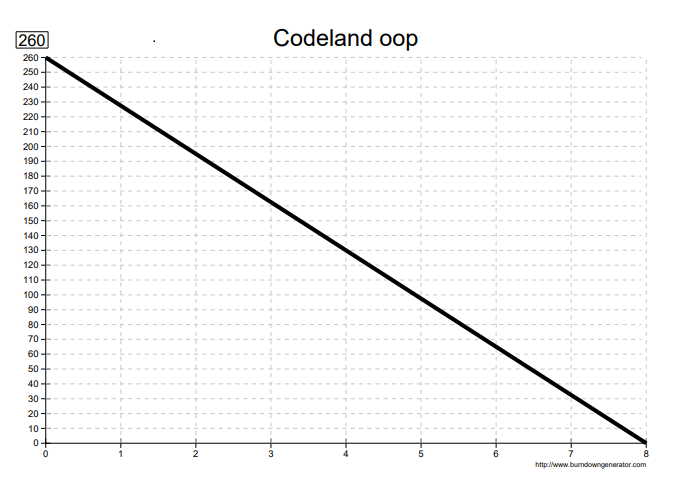
\includegraphics[scale=0.7]{img/quemado.png} 
		\caption{Grafica de quemado de las historias de usuario.}
		\label{quemado}
	\end{center}
\end{figure}
	\chapter{Resultados}

Se mostrarán las pantallas que se obtuvieron al desarrollar la aplicación.

\begin{figure}[H]
	\begin{center}
		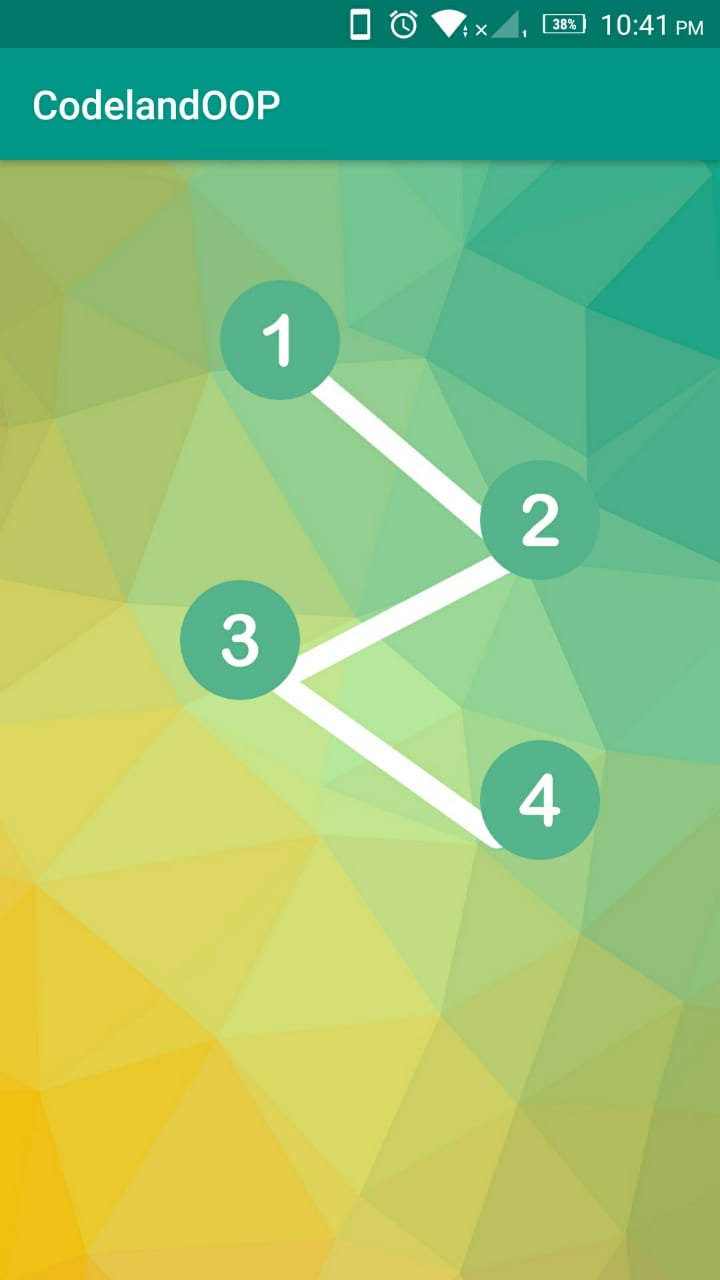
\includegraphics[scale=0.3]{img/ss1.jpeg} 
		\caption{Pantalla de inicio donde se muestran las fases.}
		\label{fases}
	\end{center}
\end{figure}

\begin{figure}[H]
	\begin{center}
		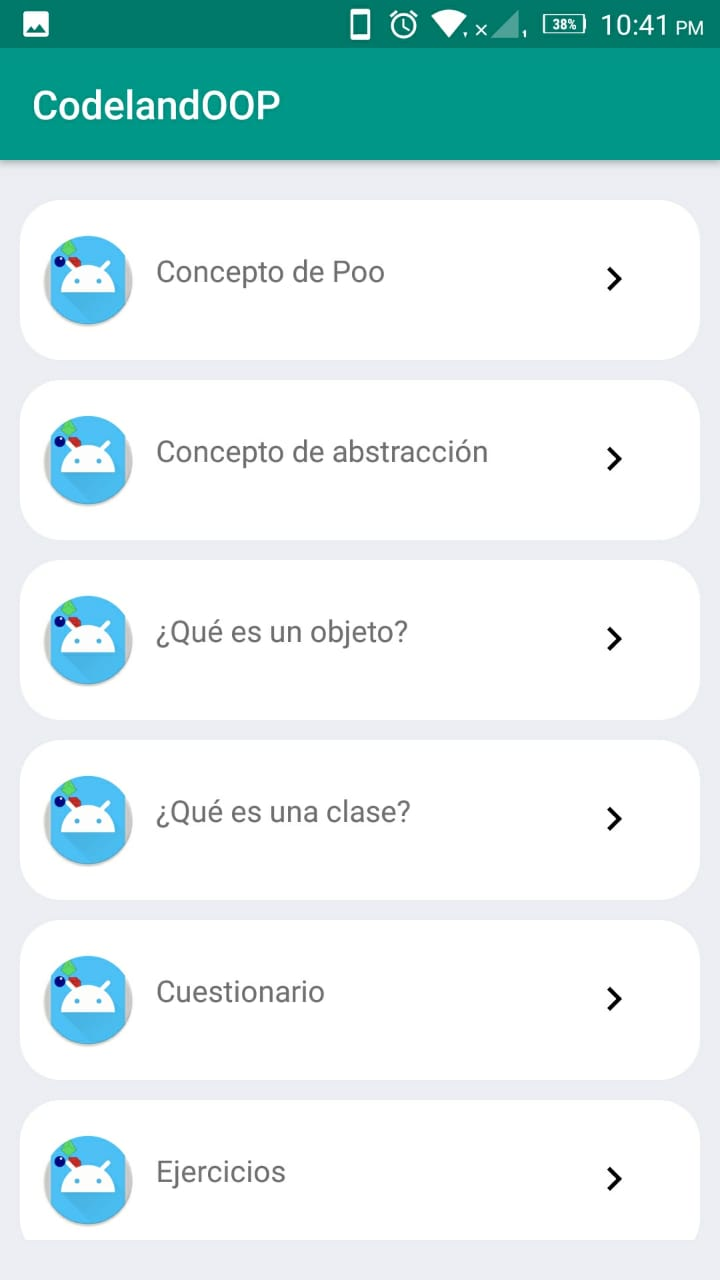
\includegraphics[scale=0.3]{img/ss2.jpeg} 
		\caption{Pantalla de selección de los temas de cada fase.}
		\label{temas}
	\end{center}
\end{figure}
	\chapter*{Anexos}

	\chapter{Mockups}

	\renewcommand{\bibname}{Referencias}
	\bibliographystyle{apalike}
	\bibliography{bibliografia}
\end{document}